\section{Конструкторская часть}

В данном разделе будет представлена структура проектируемой базы данных для фитнес-клуба, включая описание сущностей, ограничений целостности данных, а также модели ролей пользователей. Также будут описаны используемые функции, процедуры и триггеры, обеспечивающие корректность и безопасность работы с данными.

\subsection{Разработка базы данных}

На рисунке~\ref{fig:db-er} представлена схема проектируемой базы данных.

\begin{figure}[ht!]
	\begin{center}
		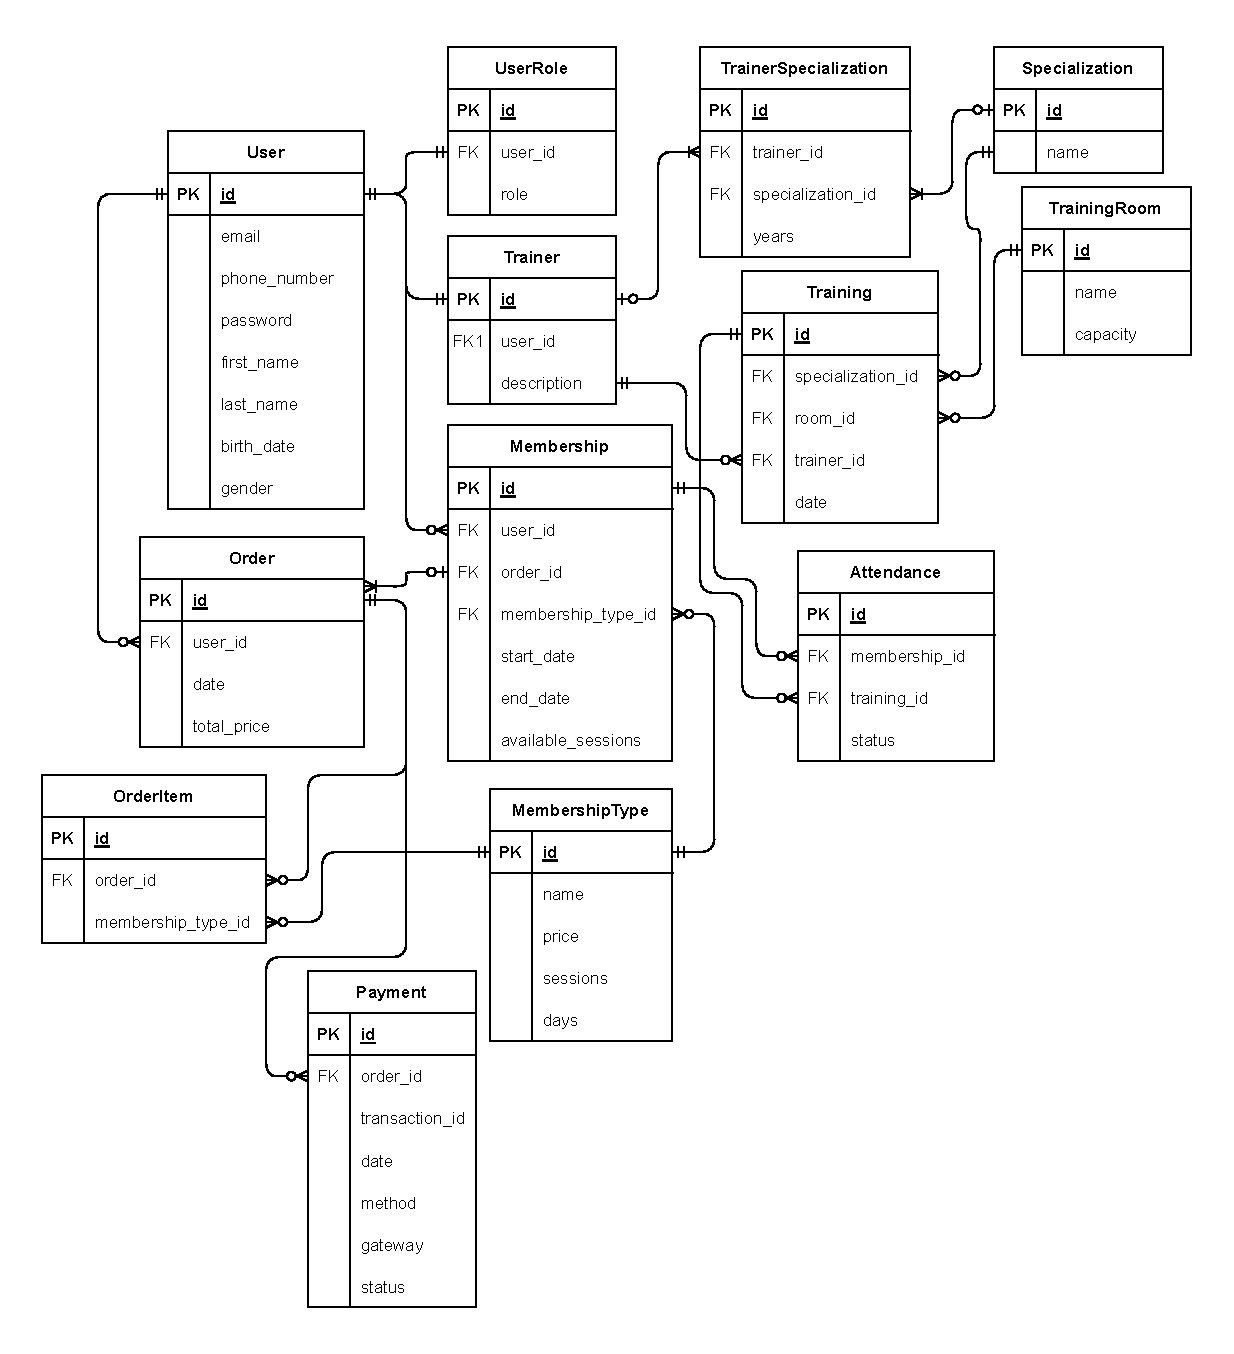
\includegraphics[scale=0.68]{./diag/db-er.pdf}
	\end{center}
	\caption{ER-диграмма базы данных фитнес-клуба}
	\label{fig:db-er}
\end{figure}

\subsection{Разработка сущностей базы данных}

Далее будут описаны тринадцать сущностей проектируемой базы данных.

\textbf{User} -- cущность, представляющая зарегистрированного пользователя системы.

Атрибуты: 
\begin{itemize} 
	\item \textit{id} -- уникальный идентификатор пользователя; 
	\item \textit{first\_name} -- имя;
	\item \textit{last\_name} -- фамилия; 
	\item \textit{email} -- адрес электронной почты;
	\item \textit{password} — зашифрованный пароль;
	\item \textit{phone\_number} — номер телефона;
	\item \textit{birth\_date} — дата рождения;
	\item \textit{gender} — пол пользователя. 
\end{itemize}

\textbf{UserRole} -- cущность, представляющая роли конкретных пользователей.

Атрибуты: 
\begin{itemize} 
	\item \textit{id} -- уникальный идентификатор роли;
	\item \textit{role} -- название роли пользователя;
	\item \textit{user\_id} -- внешний ключ, ссылающийся на пользователя.
\end{itemize}

\textbf{Trainer} -- cущность, представляющая дополнительная информацию о пользователях-тренерах.

Атрибуты: 
\begin{itemize} 
	\item \textit{id} -- уникальный идентификатор тренера;
	\item \textit{user\_id} -- внешний ключ, ссылающийся на пользователя;
	\item \textit{description} -- краткое описание или биография. 
\end{itemize}

\textbf{Specialization} -- cущность, представляющая типы специализаций тренеров и тренировок.

Атрибуты:
\begin{itemize} 
	\item \textit{id} -- уникальный идентификатор специализации; 
	\item \textit{name} -- название специализации.
\end{itemize}

\textbf{TrainerSpecialization} -- cущность, представляющая связь между тренерами и их специализациями, то есть специализации тренеров.

Атрибуты:
\begin{itemize} 
	\item \textit{id} -- уникальный идентификатор специализации тренера;
	\item \textit{trainer\_id} -- внешний ключ, ссылающийся на тренера;
	\item \textit{specialization\_id} -- внешний ключ, ссылающийся на специализацию;
	\item \textit{years} -- опыт тренера в годах для специализации.
\end{itemize}

\textbf{TrainingRoom} -- cущность, представляющая залы, в которых проводятся тренировки.

Атрибуты:
\begin{itemize} 
	\item \textit{id} -- уникальный идентификатор зала;
	\item \textit{name} -- название зала; 
	\item \textit{capacity} — вместимость зала.
\end{itemize}

\textbf{MembershipType} -- cущность, представляющая типы абонементов, доступных для покупки.

Атрибуты:
\begin{itemize} 
	\item \textit{id} -- уникальный идентификатор типа абонемента;
	\item \textit{name} -- название типа абонемента; 
	\item \textit{days} -- длительность действия в днях;
	\item \textit{price} -- стоимость;
	\item \textit{sessions} -- количество доступных тренировок.
\end{itemize}

\textbf{Membership} -- cущность, представляющая абонементы, приобретённые пользователями.

Атрибуты:
\begin{itemize} 
	\item \textit{id} -- уникальный идентификатор абонемента; 
	\item \textit{user\_id} -- внешний ключ, ссылающийся на пользователя-клиента;
	\item \textit{membership\_type\_id} -- внешний ключ, ссылающийся на тип абонемента;
	\item \textit{start\_date} -- дата начала действия;
	\item \textit{end\_date} -- дата окончания действия;
	\item \textit{available\_sessions} -- количество доступных (оставшихся) тренировок.
\end{itemize}

\textbf{Order} -- cущность, представляющая оформленные пользователями заказы.

Атрибуты:
\begin{itemize} 
	\item \textit{id} -- уникальный идентификатор заказа; 
	\item \textit{user\_id} -- внешний ключ, ссылающийся на пользователя;
	\item \textit{date} -- дата оформления;
	\item \textit{total\_price} -- общая цена заказа. 
\end{itemize}

\textbf{OrderItem} -- cущность, представляющая позиции внутри заказа.

Атрибуты:
\begin{itemize} 
	\item \textit{id} -- уникальный идентификатор позиции заказа;
	\item \textit{order\_id} -- внешний ключ, ссылающийся на заказ;
	\item \textit{membership\_type\_id} -- внешний ключ, ссылающийся тип абонемента.
\end{itemize}

\textbf{Payment} -- cущность, представляющая информацию об оплате заказов.

Атрибуты:
\begin{itemize} 
	\item \textit{id} -- уникальный идентификатор платежа; 
	\item \textit{order\_id} -- внешний ключ, ссылающийся на заказ;
	\item \textit{transaction\_id} -- идентификатор транзакции, получаемый от платежной системы;
	\item \textit{date} -- дата платежа;
	\item \textit{method} -- способ оплаты;
	\item \textit{gateway} -- платежный шлюз;
	\item \textit{status} -- статус оплаты.
\end{itemize}

\textbf{Training} -- cущность, представляющая тренировки.

Атрибуты:
\begin{itemize} 
	\item \textit{id} -- уникальный идентификатор тренировки; 
	\item \textit{trainer\_id} -- внешний ключ, ссылающийся на тренера;
	\item \textit{room\_id} -- внешний ключ, ссылающийся на зал;
	\item \textit{specialization\_id} -- внешний ключ, ссылающийся на специализацию тренировки.
\end{itemize}

\textbf{Attendance} -- cущность, представляющая записи на тренировку пользователей.

Атрибуты:
\begin{itemize} 
	\item \textbf{id} -- уникальный идентификатор записи на тренировку;
	\item \textbf{training\_id} -- внешний ключ, ссылающийся на тренировку;
	\item \textbf{user\_id} -- внешний ключ, ссылающийся пользователя-клиента; 
	\item \textbf{status} -- статус участия.
\end{itemize}

\subsection{Разработка ограничений целостности данных}

Далее в таблицах~\ref{t:ur}--\ref{t:at}, представлены ограничения целостности данных, разработанные для сущностей проектируемой базы данных.


\begin{table}[H]
	\centering
	\begin{tabular}{|p{3.5cm}|p{3.5cm}|p{8.5cm}|}
		\hline
		\textbf{Артибут}             & \textbf{Тип данных}   & \textbf{Ограничение}             \\ \hline
		id                            & UUID                  & Уникальный идентификатор         \\ \hline
		role                          & строка                  & Не NULL, значения: ('клиент', 'тренер', 'администратор'), длина до 31 символов \\ \hline
		user\_id                      & UUID                 & Внешний ключ (ссылается на User), уникальный, каскадное удаление \\ \hline
	\end{tabular}
	\caption{Ограничения атрибутов сущности UserRole}
	\label{t:ur}
\end{table}

\begin{table}[H]
	\centering
	\begin{tabular}{|p{3.5cm}|p{3.5cm}|p{8.5cm}|}
		\hline
		\textbf{Артибут}             & \textbf{Тип данных}   & \textbf{Ограничение}             \\ \hline
		id                            & UUID                 & Уникальный идентификатор         \\ \hline
		user\_id                      & UUID                 & Внешний ключ (ссылается на User), уникальный, каскадное удаление \\ \hline
		description                   & строка                  & Не NULL, длина до 511 символов   \\ \hline
	\end{tabular}
	\caption{Ограничения атрибутов сущности Trainer}
\end{table}

\begin{table}[H]
	\centering
	\begin{tabular}{|p{3.5cm}|p{3.5cm}|p{8.5cm}|}
		\hline
		\textbf{Артибут}             & \textbf{Тип данных}   & \textbf{Ограничение}             \\ \hline
		id                            & UUID                 & Уникальный идентификатор         \\ \hline
		name                          & строка                 & Не NULL, длина до 127 символов, уникальное   \\ \hline
	\end{tabular}
	\caption{Ограничения атрибутов сущности Specialization}
\end{table}

\begin{table}[H]
	\centering
	\begin{tabular}{|p{3.5cm}|p{3.5cm}|p{8.5cm}|}
		\hline
		\textbf{Артибут}             & \textbf{Тип данных}   & \textbf{Ограничение}             \\ \hline
		id                            & UUID                  & Уникальный идентификатор         \\ \hline
		name                          & строка                 & Не NULL, длина до 63 символов, уникальное                         \\ \hline
		capacity                      & целое число              & Не NULL, больше 0                \\ \hline
	\end{tabular}
	\caption{Ограничения атрибутов сущности TrainingRoom}
\end{table}

\begin{table}[H]
	\centering
	\begin{tabular}{|p{2.5cm}|p{3.5cm}|p{9.5cm}|}
		\hline
		\textbf{Артибут}             & \textbf{Тип данных}   & \textbf{Ограничение}             \\ \hline
		id                            & UUID                 & Уникальный идентификатор         \\ \hline
		name                          & строка                 & Не NULL, уникальное,  длина до 127 символов   \\ \hline
		price                         & число с фиксированной точностью               & Не NULL, больше или равно 0.0, по умолчанию 0.0     \\ \hline
		sessions                      & целое число               & Не NULL, больше 0, по умолчанию 1              \\ \hline
		days                          & целое число              & Не NULL, больше 0, по умолчанию 1              \\ \hline
	\end{tabular}
	\caption{Ограничения атрибутов сущности MembershipType}
\end{table}

\begin{table}[H]
	\centering
	\begin{tabular}{|p{4.5cm}|p{3.5cm}|p{7.5cm}|}
		\hline
		\textbf{Артибут}             & \textbf{Тип данных}   & \textbf{Ограничение}             \\ \hline
		id                            & UUID                 & Уникальный идентификатор         \\ \hline
		order\_id                     & UUID                  & Внешний ключ (ссылается на Order), каскадное удаление \\ \hline
		membership\_type\_id          & UUID                 & Внешний ключ (ссылается на MembershipType), каскадное удаление \\ \hline
	\end{tabular}
	\caption{Ограничения атрибутов сущности OrderItem}
\end{table}


\begin{table}[H]
	\centering
	\begin{tabular}{|p{2.5cm}|p{4.5cm}|p{8.5cm}|}
		\hline
		\textbf{Артибут}             & \textbf{Тип данных}   & \textbf{Ограничение}             \\ \hline
		id                            & UUID                  & Уникальный идентификатор         \\ \hline
		user\_id                      & UUID                 & Внешний ключ (ссылается на User), при удалении родительской записи в связанной таблице поле устанавливается в NULL \\ \hline
		date                          & метка времени             & Не NULL, по умолчанию текущая метка времени, значение не меньше текущей метки времени \\ \hline
		total\_price                  & число с фиксированной точностью               & Не NULL, больше или равно 0.0, значение по умолчанию 0.0     \\ \hline
	\end{tabular}
	\caption{Ограничения атрибутов сущности Order}
\end{table}

\begin{table}[H]
	\centering
	\begin{tabular}{|p{3.5cm}|p{3.5cm}|p{8.5cm}|}
		\hline
		\textbf{Артибут}             & \textbf{Тип данных}   & \textbf{Ограничение}             \\ \hline
		id                            & UUID                  & Уникальный идентификатор         \\ \hline
		email                         & строка                 & Не NULL, уникален, проверка по регулярному выражению, которое соответствует формату email (например, user@example.com), длина до 127 символов \\ \hline
		phone\_number                 & строка                 & Не NULL, уникален, проверка по регулярному выражению, которое соответствует телефонным номерам в международном формате (например, +1234567890), длина до 31 символов \\ \hline
		password                      & строка                 & Не NULL, длина до 255 символов                        \\ \hline
		first\_name                   & строка                 & Не NULL, проверка по регулярному выражению, которое позволяет только буквы (с возможным дефисом внутри имени), длина до 127 символов \\ \hline
		last\_name                    & строка                 & Не NULL, проверка по регулярному выражению, которое позволяет только буквы (с возможным дефисом внутри фамилии), длина до 127 символов \\ \hline
		birth\_date                   & дата                   & Не NULL, проверка на возраст: от 14 до 120 лет \\ \hline
		gender                        & строка                 & Не NULL, значения: ('мужской', 'женский'), длина до 31 символов \\ \hline
	\end{tabular}
	\caption{Ограничения атрибутов сущности User}
\end{table}

\begin{table}[H]
	\centering
	\begin{tabular}{|p{3.5cm}|p{3.5cm}|p{8.5cm}|}
		\hline
		\textbf{Артибут}             & \textbf{Тип данных}   & \textbf{Ограничение}             \\ \hline
		id                            & UUID                 & Уникальный идентификатор         \\ \hline
		membership\_id                & UUID                  & Внешний ключ (ссылается на Membership), каскадное удаление \\ \hline
		training\_id         & UUID                  & Внешний ключ (ссылается на TrainingSession), при удалении родительской записи в связанной таблице поле устанавливается в NULL \\ \hline
		status         & строка                 & Не NULL, длина до 63 символов, значения: ('посетил', ожидает', 'отсутствовал'), по умолчанию 'ожидает'\\ \hline
	\end{tabular}
	\caption{Ограничения атрибутов сущности Attendance}
\end{table}

\begin{table}[H]
	\centering
	\begin{tabular}{|p{3.5cm}|p{3.5cm}|p{8.5cm}|}
		\hline
		\textbf{Артибут}             & \textbf{Тип данных}   & \textbf{Ограничение}             \\ \hline
		id                            & UUID                & Уникальный идентификатор         \\ \hline
		trainer\_id                   & UUID                  & Внешний ключ (ссылается на Trainer), при удалении родительской записи в связанной таблице поле устанавливается в NULL \\ \hline
		room\_id                      & UUID                 & Внешний ключ (ссылается на TrainingRoom), при удалении родительской записи в связанной таблице поле устанавливается в NULL\\ \hline
		specialization\_id                      & UUID                 & Внешний ключ (ссылается на Specialization), при удалении родительской записи в связанной таблице поле устанавливается в NULL\\ \hline
		date                   & метка времени                & Не NULL \\ \hline
	\end{tabular}
	\caption{Ограничения атрибутов сущности Training}
\end{table}


\begin{table}[H]
	\centering
	\begin{tabular}{|p{3.5cm}|p{3.5cm}|p{8.5cm}|}
		\hline
		\textbf{Артибут}             & \textbf{Тип данных}   & \textbf{Ограничение}             \\ \hline
		id                            & UUID                 & Уникальный идентификатор         \\ \hline
		order\_id                     & UUID                & Внешний ключ (ссылается на Order), при удалении родительской записи в связанной таблице поле устанавливается в NULL \\ \hline
		transaction\_id               & строка                  & Не NULL, уникальное, длина до 255 символов                      \\ \hline
		date                          & метка времени             & Не NULL, по умолчанию текущая метка времени \\ \hline
		method                        & строка                  & Не NULL, значения: ('наличные', 'кредитная карта', 'банковский перевод'), длина до 63 символов, по умолчанию 'наличные' \\ \hline
		gateway                       & строка               & Можеть быть NULL, длина до 63 символов, по умолчанию NULL                     \\ \hline
		status                        & строка               & Не NULL, длина до 63 символов, значения: ('ожидает', 'оплачен', 'отменен'), по умолчанию 'ожидает'. \\ \hline
	\end{tabular}
	\caption{Ограничения атрибутов сущности Payment}
\end{table}

\begin{table}[H]
	\centering
	\begin{tabular}{|p{3.5cm}|p{3.5cm}|p{8.5cm}|}
		\hline
		\textbf{Артибут}             & \textbf{Тип данных}   & \textbf{Ограничение}             \\ \hline
		id                            & UUID                  & Уникальный идентификатор         \\ \hline
		trainer\_id                   & UUID                & Внешний ключ (ссылается на Trainer), каскадное удаление \\ \hline
		specialization\_id            & UUID                 & Внешний ключ (ссылается на Specialization), уникальная комбинация (trainer\_id, specialization\_id), каскадное удаление \\ \hline
		years                         & целое число                   & Не NULL, больше или равно 0      \\ \hline
	\end{tabular}
	\caption{Ограничения атрибутов сущности TrainerSpecialization}
\end{table}

\begin{table}[H]
	\centering
	\begin{tabular}{|p{4.5cm}|p{3.5cm}|p{7.5cm}|}
		\hline
		\textbf{Артибут}             & \textbf{Тип данных}   & \textbf{Ограничение}             \\ \hline
		id                            & UUID                  & Уникальный идентификатор         \\ \hline
		user\_id                      & UUID                  & Внешний ключ (ссылается на User), каскадное удаление \\ \hline
		order\_id                     & UUID                  & Внешний ключ (ссылается на Order),  при удалении родительской записи в связанной таблице поле устанавливается в NULL\\ \hline
		membership\_type\_id          & UUID                  & Внешний ключ (ссылается на MembershipType),  при удалении родительской записи в связанной таблице поле устанавливается в NULL \\ \hline
		start\_date                   & дата                  & Может быть NULL, по умолчанию NULL \\ \hline
		end\_date                     & дата                  & Может быть NULL, по умолчанию NULL, не раньше start\_date \\ \hline
		available\_sessions           & целое число               & Не NULL, больше или равно 0, по умолчанию 0 \\ \hline
	\end{tabular}
	\caption{Ограничения атрибутов сущности Membership}
	\label{t:at}
\end{table}

\subsection{Разработка ролевой модели}

Для обеспечения безопасности и разграничения доступа к данным разработанной базе данных фитнес-клуба необходимо разработать ролевую модель управления доступом.

\subsubsection*{Роли базы данных}

\begin{enumerate}[label=\arabic*.]
	\item \textbf{Гость (Guest)}
	\begin{itemize}
		\item имеет минимальные права;
		\item имеет доступ только к функциям регистрации и аутентификации;
		\item не имеет прямого доступа к таблицам базы данных.
	\end{itemize}
	
	\item \textbf{Клиент (Client)}
	\begin{itemize}
		\item является зарегистрированным и аутентифицированным пользователем системы;
		\item может оформлять и оплачивать заказы, то есть приобретать абонементы;
		\item имеет возможность записываться на тренировки, просматривать расписание и свои персональные данные;
		\item имеет доступ только к собственным записям в таблицах: \texttt{User}, \texttt{Membership}, \texttt{Order}, \texttt{OrderItem}, \texttt{Payment}, \texttt{Attendance};
		\item может просматривать публичную информацию, содержащуюся в таблицах: \texttt{Specialization}, \texttt{TrainerSpecialization}, \texttt{MembershipType}, \texttt{TrainingRoom}, \texttt{Training}.
	\end{itemize}
	
	\item \textbf{Тренер (Trainer)}
	\begin{itemize}
		\item является поднаследником клиента (наследует все его права), но обладает расширенными возможностями;
		\item имеет доступ к записям в таблицах \texttt{Training} и \texttt{Attendance}, где он указан в качестве тренера;
		\item может просматривать информацию о своих клиентах и их посещениях тренировок;
		\item имеет право изменять данные только тех тренировок (включая посещения этих тренировок), которые он проводит.
	\end{itemize}
	
	\item \textbf{Администратор (Admin)} обладает полными правами на управление базой данных.
\end{enumerate}

\subsection{Разработка функции, процедур и триггеров}

Триггер, алгоритм которого представлен на рисунке~\ref{fig:tg-upd-mem-ses}, предназначен для автоматического обновления количества доступных тренировок у абонемента пользователя в таблице Membership в зависимости от изменения статуса посещения тренировки в таблице Attendance.

Триггер, алгоритм которого представлен на рисунке~\ref{fig:tg-att-capacity}, предназначен для проверки вместимости зала перед тем, как записать пользователя на тренировку. Он предотвращает запись, если в зале нет свободных мест для выбранной тренировки.

\begin{figure}[ht!]
	\centering
	\begin{minipage}{0.48\textwidth}
		\centering
		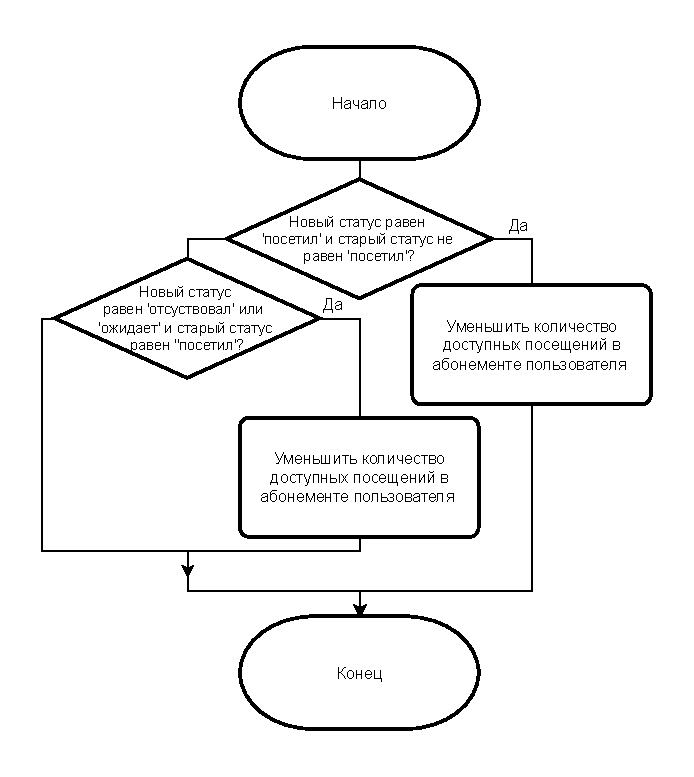
\includegraphics[scale=0.75]{./diag/trg-upd-membership-sessions.pdf}
		\caption{Схема алгоритма работы триггера для обновления данных после изменения статуса посещения тренировки}
		\label{fig:tg-upd-mem-ses}
	\end{minipage}
	\hfill
	\begin{minipage}{0.48\textwidth}
		\centering
		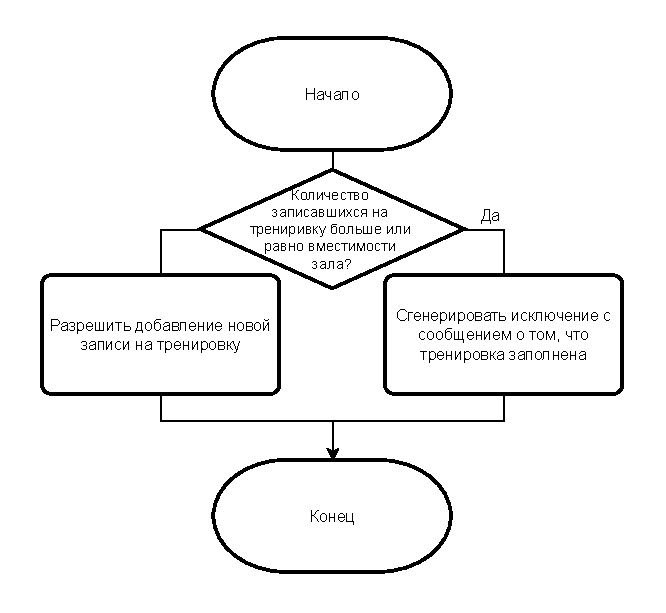
\includegraphics[scale=0.75]{./diag/trg-ins-attendance.pdf}
		\caption{Схема алгоритма работы триггера для проверки данных перед добавлением записи на тренировку}
		\label{fig:tg-att-capacity}
	\end{minipage}
\end{figure}

Триггер, алгоритм которого представлен на рисунке~\ref{fig:tg-pay}, предназначен для автоматического создания или обновления абонемента пользователя после успешного выполнения платежа. Этот триггер срабатывает, когда в таблице Payment появляется новая запись или статус платежа изменяется на <<оплачено>>.
\newpage
\begin{figure}[ht!]
	\begin{center}
		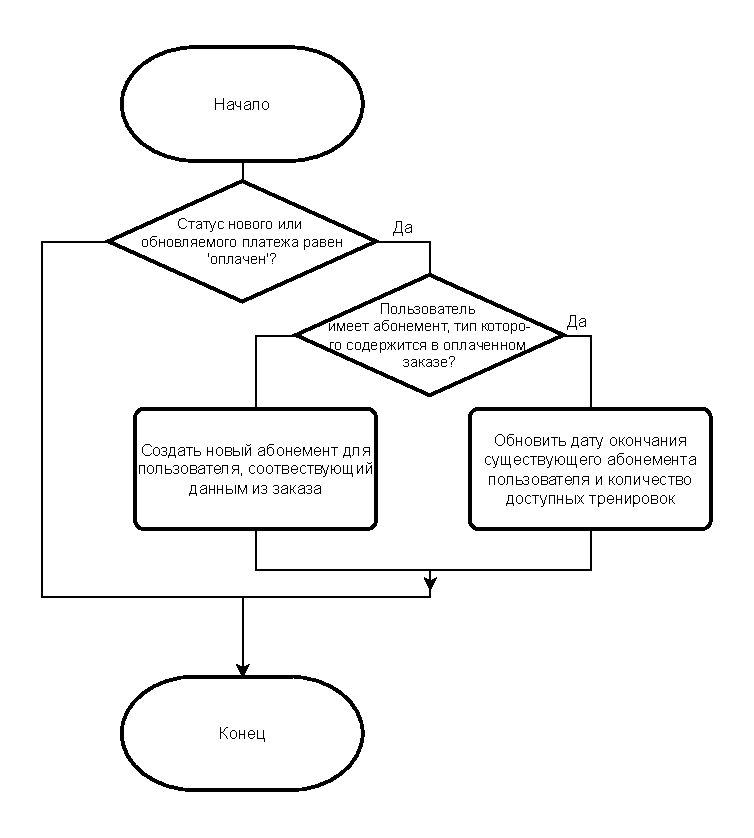
\includegraphics[scale=1]{./diag/trg-ins-upd-membership.pdf}
	\end{center}
	\caption{Схема алгоритма работы триггера для обновления или добавления данных абонемента пользователя после оплаты заказа}
	\label{fig:tg-pay}
\end{figure}

\subsection*{Вывод}

В данном разделе были разработаны база данных, ее сущности и ограничения целостности данных, а также спроектированы триггеры, обеспечивающие автоматическое обновление данных.

